\documentclass[10pt,a4paper]{article}
\usepackage[utf8]{inputenc}
\usepackage[italian]{babel}
\usepackage{amsmath}
\usepackage{amsfonts}
\usepackage{amssymb}
\usepackage[left=1cm,right=1cm,top=1cm,bottom=2cm]{geometry}
\usepackage{txfonts}
\usepackage[T1]{fontenc}
\usepackage[utf8]{inputenc}
\usepackage{graphicx}
\usepackage{wrapfig}
\usepackage{subcaption}
\usepackage{caption}
\usepackage{subcaption}
\usepackage{titlesec}
\setcounter{secnumdepth}{4}
\titleformat{\paragraph}
{\normalfont\normalsize\bfseries}{\theparagraph}{1em}{}
\titlespacing*{\paragraph}
{0pt}{3.25ex plus 1ex minus .2ex}{1.5ex plus .2ex}


\usepackage[none]{hyphenat}


\begin{document}
\subsection{Dal machine learning al deep learning}
Oggi l'intelligenza artificiale è un fiorente campo di ricerca, con l'obiettivo di risolvere una grande varietà di problemi, che per essere risolti attraverso la programmazione classica necessitano di una grande quantità di conoscenze pregresse, spesso non disponibili.\\
I Programmi basati sul paradigma dell'intelligenza artificiale si propongono di superare questi ostacoli acquisendo direttamente queste conoscenze dai dati grezzi, tale capacità è nota come machine learning.
Sotto questa famiglia di algoritmi si trovano altri sottogruppi quali il representation learning e all'interno di quest'ultimo il deep learning.\\ 
Il deep learning rispetto ai metodi più classici, tipicamente in grado di riconoscere relazioni lineari(come ad esempio il noto SVM o support vector machine), si propone come alternativa per l'apprendimento di funzioni a molte variabili non lineari anche molto complesse.
Le applicazioni più comuni comprendono il riconoscimento di oggetti nelle immagini, delle parole in tracce audio o anche per le traduzioni multilingue. \\
Il termine "deep learning" deriva proprio dalla capacità di questi modelli di riuscire a cogliere delle relazioni molto "profonde" tra i dati di ingresso e di uscita, approssimando con un certo errore ,dipendente dal caso specifico, la funzione che dati gli input restituisce l'output desiderato, purtroppo però presentano il grande problema di non rendere disponibile in maniera chiara le relazioni apprese.
   

\begin{figure}[h!]
  \centering
  \begin{subfigure}[t]{0.45\linewidth}
  	\centering
    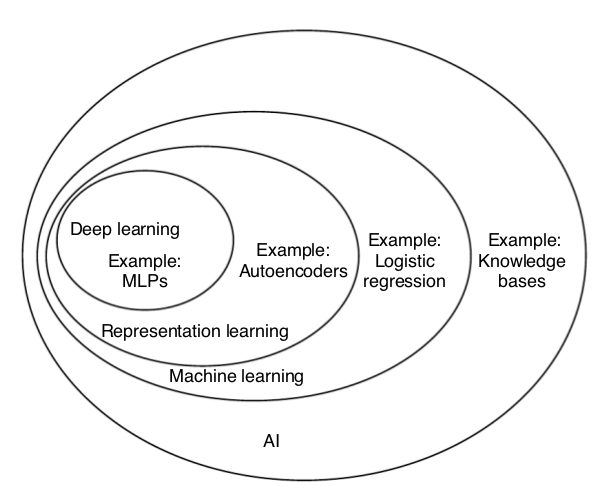
\includegraphics[height=200pt]{AI_venn_diagram.png}
    \caption*{famiglie di algoritmi}
  \end{subfigure}
  \begin{subfigure}[t]{0.45\linewidth}
  	\centering
    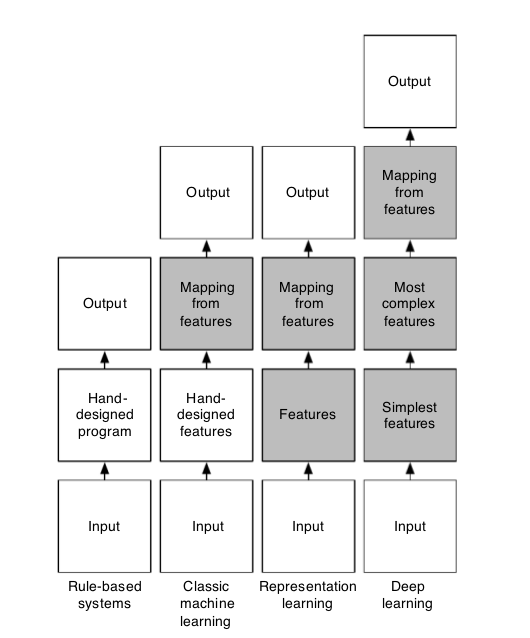
\includegraphics[height=200pt]{diff_between_aprochs.png}
    \caption*{differenze generali tra \\ le diverse tipologie di algoritmi}
  \end{subfigure}
  \label{fig:graph1}
\end{figure}

\subsubsection{Le reti feed-forward (MLP)}

\begin{wrapfigure}{r}{0.4\textwidth}
	\centering
	\vspace{-25pt}
    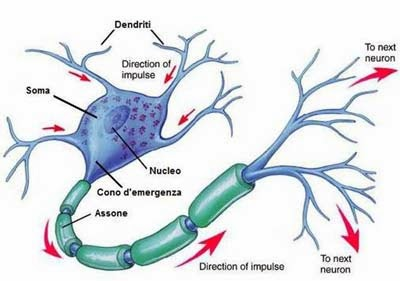
\includegraphics[width=0.4\textwidth]{neurone.jpg}
  	\caption{Il neurone biologico}
  	\label{fig:graph2}
  	\vspace{-20pt}
\end{wrapfigure}

Uno dei modelli della famiglia del deep learning più comuni e semplici da utilizzare sono le reti neurali feed-forward o multi layer perceptron, le quali sono assimilabili a modelli di regressione statistica.\\
Le reti neurali sono un modello matematico molto semplificato del\\ cervello, e per parlarne è necessario qualche riferimento al modello \\biologico.

\subsubsection*{Il neurone biologico}
L'unità base del cervello è rappresentata dai neuroni (Figuara \ref{fig:graph2}),\\ i quali a loro volta sono composti dai dendriti, dal soma, dall'assone e dalle sinapsi. 
\\I dendriti sono l'apparato di input del neurone, attraverso il quale riceve i segnali dall'ambiente o da altri neuroni, tali segnali caricano il neurone, che accumula un potenziale elettrico all'interno del soma.
In determinate condizioni o al raggiungimento di una certa soglia di potenziale il neurone emette un impulso lungo l'assone giungendo alle sinapsi, poste alla fine dell'assone, le quali sono connesse con altri neuroni o con altri apparati del corpo, come i muscoli.\\
Questa particolare cellula oltre a scambiare impulsi è in grado di accumulare informazioni attraverso l'ispessimento o l'assottigliamento della guaina mielinica, la quale è presente lungo l'assone.
Le variazioni dello spessore della guaina comportano un aumento o una diminuzione della resistenza elettrica dell'assone determinando una variazione dell'impulso percepito dai neuroni connessi alle sinapsi a parità di potenziale rilasciato.   

\newpage

\subsubsection*{Il percettrone} 

\begin{wrapfigure}{r}{0.4\textwidth}
	\centering
	\vspace{-15pt}
    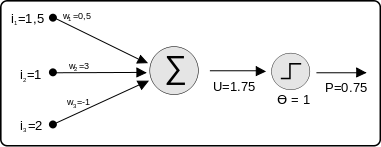
\includegraphics[width=0.4\textwidth]{percettrone.png}
  	\caption{Il percettrone}
  	\label{fig:graph3}
\end{wrapfigure}

Il neurone artificiale è composto da una serie di connessioni in ingresso, come i dendriti nel caso del neurone biologico, questa volta però il compito di immagazzinare informazione viene svolto da queste connessioni in input e non più dalle connessioni in output. 
Ad ogni input del neurone è associato un coefficiente che moltiplica il potenziale in ingresso, a questo punto gli ingressi pesati giungono al nodo sommatore, il corrispettivo del soma, che ne accumula la sommatoria.
Lo step successivo è il blocco contenente la funzione di trasferimento, una funzione che prende in input il potenziale del neurone e rende disponibile il risultato come output finale o come input per i neuroni successivi.
La funzione di trasferimento del neurone può essere di vari tipi, può variare infatti anche tra i neuroni della medesima rete, alcune delle più comuni \\sono:
\begin{wrapfigure}{r}{0.4\textwidth}
	\centering
	\vspace{-120pt}
    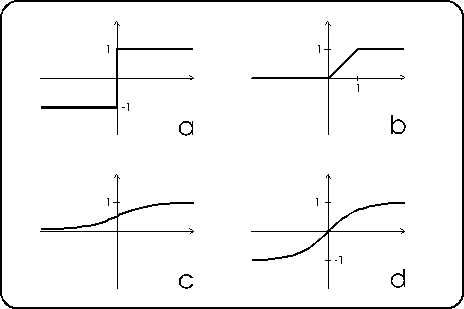
\includegraphics[width=0.4\textwidth]{FDTs.png}
  	\caption{Le funzioni di trasferimento}
  	\label{fig:graph4}
\end{wrapfigure}
(a) la funzione gradino. \\
(b) la funzione lineare con saturazione \\
(c) la funzione sigmoide tra 0 e 1 \\
(d) la funzione sigmoide tra -1 e 1 \\ \\
Volendo esprimere il percettrone in termini matematici si ottiene la seguente \\ equazione:

$\hspace*{100pt} y = f(P) = f(\textstyle\sum_i W_i \cdot X_i)$\\
\(\mathnormal{y}\) - output del percettrone\\
\(\mathnormal{f}\) - funzione di trasferimento del percettrone\\
P - potenziale del neurone\\
\(W_i\) - peso o coefficiente dell'i-esimo ingresso\\
\(X_i\) - potenziale d'ingresso dell'i-esimo neurone\\
\\Una delle caratteristiche più importanti del percettrone è la sua capacità di compiere separazioni lineari. Tali separazioni avvengono in uno spazio a n dimensioni, dove n corrisponde al numero di variabili in ingresso al neurone, perciò si avrà ad esempio per un percettrone a due input la capacita di separare i valori su \(\Re^2\) attraverso un retta, nel caso \(\Re^3\) si potranno separare i valori dello spazio tridimensionale attraverso un piano, e così via.\\
\begin{figure}[h!]
  \centering
  \begin{subfigure}[t]{0.45\linewidth}
  	\centering
  	%\hspace{-120pt}
    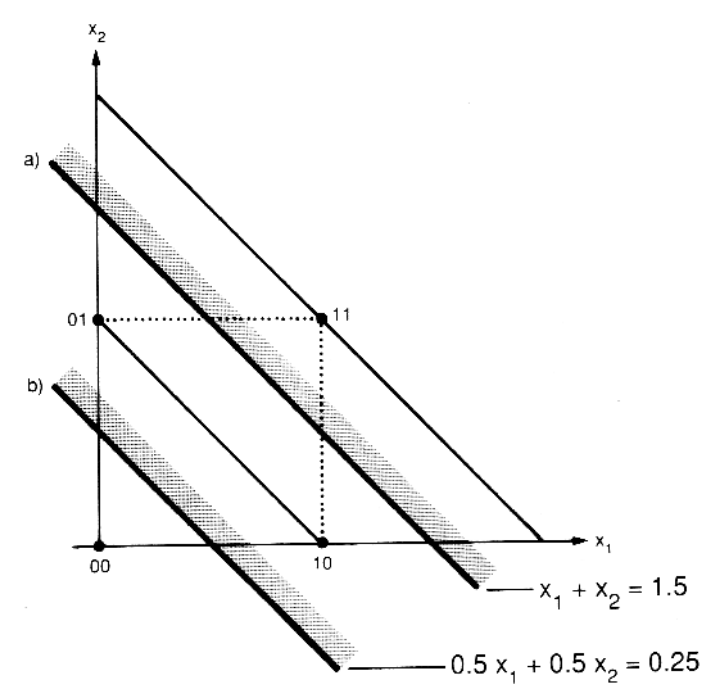
\includegraphics[height=240pt]{sepAndOr.png}
    \captionsetup{justification=centering}
    \caption*{esempio di linee di separazione per neurone a 2 ingressi binari\\
    (a - funzione OR)\\
    (b - funzione AND)}
  \end{subfigure}
  \begin{subfigure}[t]{0.45\linewidth}
    %\hspace{-200pt}
  	\centering
    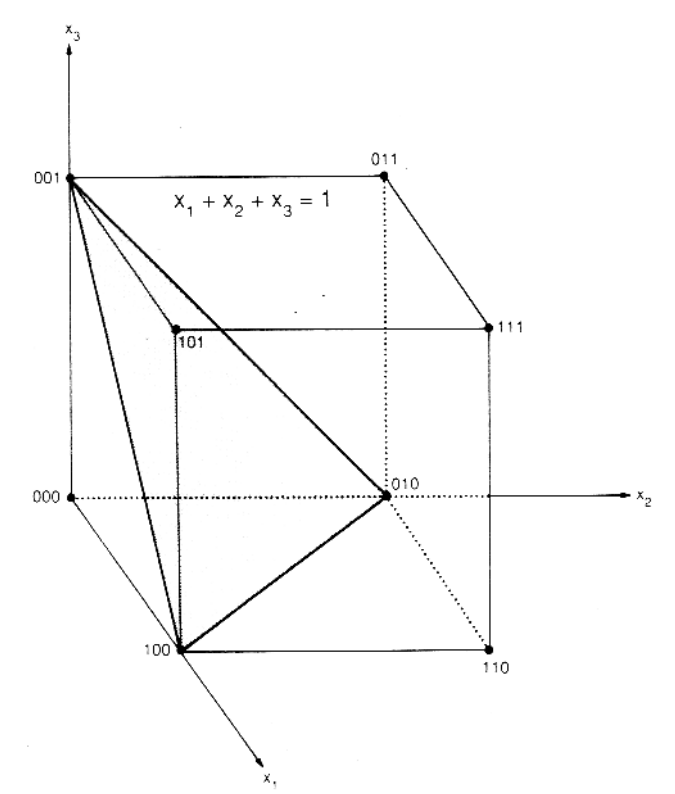
\includegraphics[height=240pt]{sepR3.png}
    \captionsetup{justification=centering}
    \caption*{esempio di piano diseparazione lineare \\ a 3 ingressi per un neurone binario}
  \end{subfigure}
  \label{fig:graph5}
\end{figure}
\\ \\

\subsubsection*{Il problema dello XOR}
 
\subsubsection*{Le reti multi-strato e la separazione non lineare} 
Le reti multi strato sono composte da strati di percettroni, interconnessi tra loro in modo che gli output degli strati precedenti siano connessi con gli input dei percettorini successivi.
 
\subsubsection{La funzione di addestramento: Il back-propagation} 

\end{document}